\documentclass[11pt]{article}

\usepackage[margin=1in]{geometry}
\usepackage[utf8]{inputenc}
\usepackage[T1]{fontenc}
\usepackage{booktabs}
\usepackage{graphicx}
\usepackage{amsmath}
\usepackage{amssymb}
\usepackage{microtype}
\usepackage{pgfplots}
\pgfplotsset{compat=1.17}
\usepackage[numbers,sort&compress]{natbib}
\usepackage{hyperref}

% Generated from the frozen SG-000023 evidence package; never edit these by hand.
% Generated by tools/build_sg000024_manuscript_inputs.py; do not edit.
% Every value is copied from registry/p08_sg000023_paper_evidence and formatted for display.
\makeatletter
\newcommand{\dalnum}[1]{\ifcsname dalnum@#1\endcsname\csname dalnum@#1\endcsname\else\PackageError{dal}{Undefined DAL number #1}{}\fi}
\expandafter\def\csname dalnum@errors.all-systems-correct\endcsname{260}
\expandafter\def\csname dalnum@errors.all-systems-wrong\endcsname{219}
\expandafter\def\csname dalnum@errors.both-abstain-on-sufficient\endcsname{0}
\expandafter\def\csname dalnum@errors.both-unsafe-on-insufficient\endcsname{289}
\expandafter\def\csname dalnum@errors.paper-control-correct-laya-wrong\endcsname{16}
\expandafter\def\csname dalnum@errors.paper-control-wrong-laya-correct\endcsname{5}
\expandafter\def\csname dalnum@errors.paper-only-unsafe-on-insufficient\endcsname{211}
\expandafter\def\csname dalnum@errors.perstratum\endcsname{3}
\expandafter\def\csname dalnum@fhir.goldrows\endcsname{0}
\expandafter\def\csname dalnum@fhir.interfacefailures\endcsname{173}
\expandafter\def\csname dalnum@fhir.requested\endcsname{173}
\expandafter\def\csname dalnum@fhir.systems\endcsname{3}
\expandafter\def\csname dalnum@native.clinical_control.aurc\endcsname{0.5935}
\expandafter\def\csname dalnum@native.clinical_control.completed\endcsname{1000}
\expandafter\def\csname dalnum@native.clinical_control.failed\endcsname{0}
\expandafter\def\csname dalnum@native.clinical_control.presentactionaccuracy\endcsname{0.5520}
\expandafter\def\csname dalnum@native.clinical_control.requested\endcsname{1000}
\expandafter\def\csname dalnum@native.clinical_control.riskat50\endcsname{0.6040}
\expandafter\def\csname dalnum@native.clinical_control.riskat80\endcsname{0.6675}
\expandafter\def\csname dalnum@native.clinical_control.riskat90\endcsname{0.6967}
\expandafter\def\csname dalnum@native.clinical_control.target05.actualcoverage\endcsname{0.4910}
\expandafter\def\csname dalnum@native.clinical_control.target05.overabstainrate\endcsname{0.2720}
\expandafter\def\csname dalnum@native.clinical_control.target05.threshold\endcsname{0.5343}
\expandafter\def\csname dalnum@native.clinical_control.target05.unsafecommitrate\endcsname{0.2540}
\expandafter\def\csname dalnum@native.clinical_control.target08.actualcoverage\endcsname{0.7690}
\expandafter\def\csname dalnum@native.clinical_control.target08.overabstainrate\endcsname{0.0400}
\expandafter\def\csname dalnum@native.clinical_control.target08.threshold\endcsname{0.5109}
\expandafter\def\csname dalnum@native.clinical_control.target08.unsafecommitrate\endcsname{0.5780}
\expandafter\def\csname dalnum@native.clinical_control.target09.actualcoverage\endcsname{0.8520}
\expandafter\def\csname dalnum@native.clinical_control.target09.overabstainrate\endcsname{0.0200}
\expandafter\def\csname dalnum@native.clinical_control.target09.threshold\endcsname{0.5001}
\expandafter\def\csname dalnum@native.clinical_control.target09.unsafecommitrate\endcsname{0.7240}
\expandafter\def\csname dalnum@native.diff.cihigh\endcsname{-0.0050}
\expandafter\def\csname dalnum@native.diff.cilow\endcsname{-0.0200}
\expandafter\def\csname dalnum@native.diff.estimate\endcsname{-0.0125}
\expandafter\def\csname dalnum@native.identity.correctness\endcsname{1000}
\expandafter\def\csname dalnum@native.identity.rows\endcsname{1000}
\expandafter\def\csname dalnum@native.identity.scores\endcsname{0}
\expandafter\def\csname dalnum@native.laya.aurc\endcsname{--}
\expandafter\def\csname dalnum@native.laya.completed\endcsname{0}
\expandafter\def\csname dalnum@native.laya.failed\endcsname{1000}
\expandafter\def\csname dalnum@native.laya.presentactionaccuracy\endcsname{--}
\expandafter\def\csname dalnum@native.laya.requested\endcsname{1000}
\expandafter\def\csname dalnum@native.laya.riskat50\endcsname{--}
\expandafter\def\csname dalnum@native.laya.riskat80\endcsname{--}
\expandafter\def\csname dalnum@native.laya.riskat90\endcsname{--}
\expandafter\def\csname dalnum@native.paper.aurc\endcsname{0.5296}
\expandafter\def\csname dalnum@native.paper.completed\endcsname{1000}
\expandafter\def\csname dalnum@native.paper.failed\endcsname{0}
\expandafter\def\csname dalnum@native.paper.presentactionaccuracy\endcsname{0.5520}
\expandafter\def\csname dalnum@native.paper.requested\endcsname{1000}
\expandafter\def\csname dalnum@native.paper.riskat50\endcsname{0.4480}
\expandafter\def\csname dalnum@native.paper.riskat80\endcsname{0.6550}
\expandafter\def\csname dalnum@native.paper.riskat90\endcsname{0.6933}
\expandafter\def\csname dalnum@native.paper.target05.actualcoverage\endcsname{0.4920}
\expandafter\def\csname dalnum@native.paper.target05.overabstainrate\endcsname{0.0160}
\expandafter\def\csname dalnum@native.paper.target05.threshold\endcsname{0.9998}
\expandafter\def\csname dalnum@native.paper.target05.unsafecommitrate\endcsname{0.0000}
\expandafter\def\csname dalnum@native.paper.target08.actualcoverage\endcsname{1.0000}
\expandafter\def\csname dalnum@native.paper.target08.overabstainrate\endcsname{0.0000}
\expandafter\def\csname dalnum@native.paper.target08.threshold\endcsname{0.0000}
\expandafter\def\csname dalnum@native.paper.target08.unsafecommitrate\endcsname{1.0000}
\expandafter\def\csname dalnum@native.paper.target09.actualcoverage\endcsname{1.0000}
\expandafter\def\csname dalnum@native.paper.target09.overabstainrate\endcsname{0.0000}
\expandafter\def\csname dalnum@native.paper.target09.threshold\endcsname{0.0000}
\expandafter\def\csname dalnum@native.paper.target09.unsafecommitrate\endcsname{1.0000}
\expandafter\def\csname dalnum@pubmedqa.bootstrap.replicates\endcsname{10000}
\expandafter\def\csname dalnum@pubmedqa.bootstrap.seed\endcsname{1729}
\expandafter\def\csname dalnum@pubmedqa.clinical_control.accuracy\endcsname{0.5520}
\expandafter\def\csname dalnum@pubmedqa.clinical_control.completed\endcsname{500}
\expandafter\def\csname dalnum@pubmedqa.clinical_control.ece_15_equal_width\endcsname{0.0360}
\expandafter\def\csname dalnum@pubmedqa.clinical_control.macro_f1\endcsname{0.2371}
\expandafter\def\csname dalnum@pubmedqa.clinical_control.multiclass_brier\endcsname{0.5695}
\expandafter\def\csname dalnum@pubmedqa.clinical_control.nll\endcsname{0.9385}
\expandafter\def\csname dalnum@pubmedqa.clinical_control.requested\endcsname{500}
\expandafter\def\csname dalnum@pubmedqa.diff.cihigh\endcsname{0.0000}
\expandafter\def\csname dalnum@pubmedqa.diff.cilow\endcsname{0.0000}
\expandafter\def\csname dalnum@pubmedqa.diff.estimate\endcsname{0.0000}
\expandafter\def\csname dalnum@pubmedqa.identity.probabilities\endcsname{500}
\expandafter\def\csname dalnum@pubmedqa.identity.rows\endcsname{500}
\expandafter\def\csname dalnum@pubmedqa.laya.accuracy\endcsname{0.5300}
\expandafter\def\csname dalnum@pubmedqa.laya.completed\endcsname{500}
\expandafter\def\csname dalnum@pubmedqa.laya.ece_15_equal_width\endcsname{--}
\expandafter\def\csname dalnum@pubmedqa.laya.macro_f1\endcsname{--}
\expandafter\def\csname dalnum@pubmedqa.laya.multiclass_brier\endcsname{0.6805}
\expandafter\def\csname dalnum@pubmedqa.laya.nll\endcsname{1.1976}
\expandafter\def\csname dalnum@pubmedqa.laya.requested\endcsname{500}
\expandafter\def\csname dalnum@pubmedqa.paper.accuracy\endcsname{0.5520}
\expandafter\def\csname dalnum@pubmedqa.paper.completed\endcsname{500}
\expandafter\def\csname dalnum@pubmedqa.paper.ece_15_equal_width\endcsname{0.0360}
\expandafter\def\csname dalnum@pubmedqa.paper.macro_f1\endcsname{0.2371}
\expandafter\def\csname dalnum@pubmedqa.paper.multiclass_brier\endcsname{0.5695}
\expandafter\def\csname dalnum@pubmedqa.paper.nll\endcsname{0.9385}
\expandafter\def\csname dalnum@pubmedqa.paper.requested\endcsname{500}
\makeatother

% Generated by tools/build_sg000024_manuscript_inputs.py; do not edit.
% \dalclaim{ID} expands to the frozen permitted wording of an affirmative claim.
% \dallimitation{ID} expands to the frozen wording of a limitation statement.
\makeatletter
\newcommand{\dalclaim}[1]{\ifcsname dalclaim@#1\endcsname\csname dalclaim@#1\endcsname\else\PackageError{dal}{#1 is not an exportable frozen claim}{}\fi}
\newcommand{\dallimitation}[1]{\ifcsname dallimitation@#1\endcsname\csname dallimitation@#1\endcsname\else\PackageError{dal}{#1 is not a frozen limitation statement}{}\fi}
\expandafter\def\csname dalclaim@SG23-C001\endcsname{On the frozen PubMedQA PQA-L final rows, the paper system achieved action accuracy 0.552 and the clinical control achieved action accuracy 0.552.}
\expandafter\def\csname dalclaim@SG23-C002\endcsname{The frozen paper-minus-control PubMedQA action-accuracy estimate is 0.0000 with a 95\% paired-bootstrap interval [0.0000, 0.0000]; this does not support a superiority claim.}
\expandafter\def\csname dalclaim@SG23-C003\endcsname{Laya completed 500 of 500 frozen PubMedQA rows with action accuracy 0.53; affected Laya confidence is excluded from reliability/calibration figures as uncalibrated.}
\expandafter\def\csname dalclaim@SG23-C004\endcsname{At the frozen native target-coverage 0.8 policy, the paper system achieved actual coverage 1.0 with unsafe-commit rate 1.0, while the clinical control achieved actual coverage 0.769 with unsafe-commit rate 0.578.}
\expandafter\def\csname dalclaim@SG23-C005\endcsname{Frozen native risk@80 is 0.655 for the paper system and 0.6675 for the clinical control (paper-minus-control estimate -0.0125, 95\% paired-bootstrap interval [-0.0200, -0.0050], lower is better); this is descriptive and is not exported as a superiority claim.}
\expandafter\def\csname dalclaim@SG23-C006\endcsname{FHIR-AgentBench final action selection is blocked pre-execution because the frozen adapter cannot represent variable candidate action sets; 0 gold rows were loaded for a requested denominator of 173, and no replacement adapter is permitted.}
\expandafter\def\csname dallimitation@SG23-C007\endcsname{Medical evidence-intervention effectiveness is not supported because canonical P06 evidence is synthetic/mechanics-only.}
\expandafter\def\csname dallimitation@SG23-C008\endcsname{Preregistered distribution-shift slice effects are unavailable because no valid frozen slice semantics are bound to final rows.}
\expandafter\def\csname dallimitation@SG23-C009\endcsname{Direct latency, throughput, and peak-memory superiority are not supported by the canonical final evidence.}
\expandafter\def\csname dallimitation@SG23-C010\endcsname{Superiority, clinical safety, SOTA, final FHIR performance, and direct efficiency superiority are not claimed.}
\expandafter\def\csname dallimitation@SG23-C011\endcsname{After the 2026-10-01 related-work refresh, these novelty claims are removed: first medical abstention system or benchmark; first clinical uncertainty, assurance, or governance layer; first typed-decision or System-One evaluation in medicine or on PubMedQA; typed non-generative readout improves medical accuracy; first pre-registered or frozen-protocol typed-decision evaluation; first deterministic hash-verified provenance for paper numbers, or first evidence/claim ledger; FHIR-aware decision-layer capability; medical counterfactual or evidence-intervention robustness. Narrowed to descriptive reporting with no directional superiority claim: superiority of native abstention over the confidence-only control (risk@80 paper-minus-control -0.0125 (95\% paired-bootstrap interval [-0.0200, -0.0050]) is descriptive under the frozen protocol; frozen 0.8 and 0.9 target policies yielded coverage 1.0 and unsafe-commit rate 1.0).}
\expandafter\def\csname dalclaim@SG23-C012\endcsname{This study reports a frozen-protocol evaluation in which every exported claim is bound to source-hashed evidence packets and null, negative, and blocked outcomes are reported. We do not claim methodological novelty for abstention, typed decisions, pre-registration, or provenance verification individually.}
\expandafter\def\csname dallimitation@SG23-C013\endcsname{An ECAL benefit is not established: the frozen selection kept evidence for compatibility with the frozen paper checkpoint rather than for a measured ablation benefit, canonical P04 paper decisions are defer-real-data, and no final-test ECAL ablation exists.}
\expandafter\def\csname dalclaim@SG23-C014\endcsname{The paper system and the clinical control emitted identical action-probability vectors on 500 of 500 frozen PubMedQA rows and identical action correctness on 1000 of 1000 native-abstention rows; the compared systems differ in selection scores (0 identical score rows), so the PubMedQA comparison isolates no action-selection difference.}
\makeatother


% Manuscript rules (enforced by tests/test_p09_sg000024_manuscript.py):
% - every result value is a \dalnum{...} macro generated from frozen evidence;
% - every claim sentence is a \dalclaim{...} (affirmative) or \dallimitation{...} macro;
% - every citation key exists in generated/references.bib.

\title{A Frozen-Protocol Evaluation of a Decision Assurance Layer for Clinical Typed Decisions:\\
Null Accuracy, Descriptive Abstention, and Blocked Interoperability Results}
\author{Author list to be confirmed by the project founder before submission}
\date{}

\begin{document}
\maketitle

\begin{abstract}
We report a single frozen-protocol evaluation of DAL, a Decision Assurance Layer that adds an
information-sufficiency signal to a compact, non-generative clinical typed-decision model without
changing that model's action distribution. All model, calibration, threshold, benchmark, and
statistics choices were fixed before final-test access, and the final evaluation ran once.
\dalclaim{SG23-C001} \dalclaim{SG23-C014} \dalclaim{SG23-C005} \dalclaim{SG23-C004}
\dalclaim{SG23-C006} The paper contributes an evaluation record, not a new method:
\dalclaim{SG23-C012}
\end{abstract}

\section{Introduction}

Many clinical decision-support workflows end in a bounded choice: select one of a small number of
allowed actions, or decline to act because the available information is insufficient. Typed-decision
(``System One'') models return a probability distribution over caller-defined options rather than free
text~\citep{jev_blog,laya_repo,decider_repo,clm_repo}. For such models, the most probable option is not by itself
permission to act. A separate signal is needed that says whether the evidence in hand supports any
decision at all.

DAL (Decision Assurance Layer) studies that separation. Its paper system keeps the action
distribution of a matched clinical encoder exactly and adds a learned information-sufficiency head
that is used only to decide whether to commit. This paper reports what a single, prospectively frozen
evaluation of that design shows, including null, negative, and blocked outcomes.

We emphasize what the evaluation does \emph{not} show. It does not establish an accuracy benefit, a
selective-risk superiority claim, clinical safety, or FHIR capability, and the 2026 literature already
covers medical abstention, typed-decision evaluation, and deterministic provenance checking
(Section~\ref{sec:related}). Our contribution is the evaluation record itself: every exported claim is
bound to a source-hashed evidence packet, and unfavorable outcomes are reported in full.

\section{Related Work}
\label{sec:related}

\paragraph{Medical abstention and selective prediction.}
MedQAbstain~\citep{cocchieri2026medqabstain} and MedAbstain~\citep{arxiv2601_12471} benchmark abstention in medical
multiple-choice settings, AbstentionBench~\citep{arxiv2506_09038} does so across domains, and a recent review
frames healthcare abstention decision-theoretically~\citep{presacan2026silence}. MedBayes-Lite~\citep{arxiv2511_16625}
describes a retraining-free clinical uncertainty governance layer. Further work documents overconfidence
under missing clinical information~\citep{arxiv2608_09080}, selective prediction on medical text~\citep{arxiv2502_18050},
knowledge-driven clinical abstention~\citep{arxiv2509_24816}, and agent-level abstention~\citep{arxiv2607_10059,arxiv2606_28733}.
We follow established selective-classification methodology~\citep{geifman2017selective,arxiv2407_01032,arxiv2410_15361}.

\paragraph{Typed-decision models.}
Concurrent studies evaluate typed-decision models in medicine~\citep{arxiv2609_34024}, test the coherence of
their probabilities~\citep{arxiv2609_33209}, evaluate them for selective automation~\citep{arxiv2609_33401}, and run
pre-registered studies with them~\citep{arxiv2609_34227}. An early evidence audit reports that the typed readout
has not shown an independent accuracy advantage over comparable label-probability readouts~\citep{arxiv2609_32160}.

\paragraph{Clinical encoders, FHIR, and healthcare agents.}
DAL builds on BioClinical ModernBERT~\citep{sounack2025bioclinicalmodernbert}; Clinical ModernBERT is a related
encoder~\citep{lee2025clinicalmodernbert}. Interoperable EHR evaluation includes FHIR-AgentBench~\citep{lee2026fhiragentbench},
MedAgentBench~\citep{jiang2025medagentbench}, HealthAgentBench~\citep{arxiv2606_31179}, FHIRPath-QA~\citep{arxiv2602_23479},
CliniCARE-Bench~\citep{arxiv2608_07796}, reinforcement learning for FHIR tool calling~\citep{arxiv2605_14126}, and a study
showing that FHIR serialization changes model behavior~\citep{arxiv2604_21076}.

\paragraph{Evidence grounding, calibration, and counterfactuals.}
Evidence verification and attribution are studied by Med-PRM~\citep{yun2025medprm}, MedTrust-RAG~\citep{arxiv2510_14400},
Med-V1~\citep{arxiv2603_05308}, and EHRNote-ChatQA~\citep{arxiv2606_15735}. Calibration of medical language models is
benchmarked in~\citep{arxiv2506_10769,boie2026calibration}, building on~\citep{guo2017calibration,gneiting2007proper}. Real-data
clinical counterfactual robustness is benchmarked by MamaBench~\citep{arxiv2607_14385}.

\paragraph{Evaluation governance and provenance.}
Deterministic integrity gates with content-hash manifests have been proposed for LLM-assisted clinical
manuscripts~\citep{arxiv2606_09500}, and evidence ledgers for governance and agent reasoning~\citep{arxiv2607_05410,arxiv2607_28374}.
Our claim-to-evidence binding is engineering practice in this study, not a new method.

\paragraph{Novelty disposition.}
A dated related-work refresh (2026-10-01; Appendix~\ref{app:literature}) removed every first-of-kind claim we had
considered: \dallimitation{SG23-C011}

\section{The Decision Assurance Layer}
\label{sec:method}

\paragraph{Typed decision interface.}
Each item offers a closed set of candidate actions (for PubMedQA: \emph{yes}, \emph{no}, \emph{maybe}).
A system returns a probability distribution over those actions and, separately, a selection score that
decides whether to commit. \emph{Abstain} is never an action; it is the decision not to commit.

\paragraph{Architecture.}
The paper system is the final development architecture (D03, ``shadow assurance critic''). The matched
clinical control is a BioClinical ModernBERT encoder with a linear action head, trained and selected
independently for each seed. DAL clones the selected same-seed control head and freezes it, so DAL's
action probabilities equal the control's exactly by construction. DAL then trains six assurance
scalars: a typed evidence-critic residual scale, three critic class biases, and the scale and bias of an
information-sufficiency head driven by the evidence-delta norm. These signals never modify the action
distribution. Two earlier development architectures (D01, D02), which did alter the action head, were
rejected on development data before D03 was frozen; no further architecture search was permitted.

\paragraph{Calibration.}
Action probabilities use scalar temperature scaling and the sufficiency score uses Platt scaling, both
fit on calibration rows only (method \texttt{temperature-scaling-action+platt-sufficiency-v0.1}). Target
coverages $0.50$, $0.80$, and $0.90$ and their thresholds were frozen before final-test access.

\paragraph{ECAL.}
Evidence-Calibrated Action Learning (ECAL) was implemented as a controlled-ablation framework, but no
paper-level ECAL benefit was measured. \dallimitation{SG23-C013} Table~\ref{tab:ecal} lists the frozen selection.

\section{Frozen Protocol and Benchmarks}
\label{sec:protocol}

\paragraph{Governance.}
Each step, from protocol freeze through final-test authorization, the one-shot final evaluation,
evidence promotion, and the post-final analysis, was a separately reviewed change with exact-revision
continuous integration on Linux and Windows and Python 3.11 and 3.12, plus two automated
code-review gates. Final-test access stayed sealed until a digest-bound authorization artifact was merged,
and the final evaluation ran exactly once. Results were not used to change any model, threshold,
calibration, benchmark, or statistic.

\paragraph{Benchmarks.}
\emph{PubMedQA PQA-L}~\citep{jin2019pubmedqa}: of its 1000 expert-labeled records, 500 form the frozen final test,
450 were used for training and development selection, and 50 for calibration. \emph{Native abstention}: each
final-test PubMedQA item appears twice, once with its evidence context present (gold: sufficient) and once with
the evidence withheld (gold: insufficient, no gold action). Withheld rows count as incorrect actions for every
system, so selective risk measures whether a selection score commits to evidence-present items. This is a
constructed evidence-availability intervention, not real-world clinical insufficiency. DAL's selection score
is its calibrated sufficiency probability; the clinical control's is its maximum action probability.
\emph{FHIR-AgentBench}~\citep{lee2026fhiragentbench}: the frozen FHIR-AgentBench split.

\paragraph{Systems.}
The primary comparison is the DAL paper system versus the matched clinical control. Laya~\citep{laya_repo} is the
required open typed-decision baseline.

\paragraph{Statistics.}
The primary comparisons use a paired bootstrap with \dalnum{pubmedqa.bootstrap.replicates} replicates (seed
\dalnum{pubmedqa.bootstrap.seed}) and 95\% percentile intervals. No primary $p$-value construction was
preregistered, so none is reported, and no significance claim is made.

\section{Results}
\label{sec:results}

\subsection{Action selection on PubMedQA}

Table~\ref{tab:main} reports the frozen final rows. \dalclaim{SG23-C001} \dalclaim{SG23-C002}
\dalclaim{SG23-C014} \dalclaim{SG23-C003}

% Generated by tools/build_sg000024_manuscript_inputs.py; do not edit.
\begin{table}[t]
\centering
\small
\caption{PubMedQA action selection on the frozen final rows.}
\label{tab:main}
\begin{tabular}{lrrrrrr}
\toprule
System & Completed & Accuracy & Macro-F1 & NLL & Brier & ECE (15 bins) \\
\midrule
DAL paper system & 500/500 & 0.5520 & 0.2371 & 0.9385 & 0.5695 & 0.0360 \\
Clinical control & 500/500 & 0.5520 & 0.2371 & 0.9385 & 0.5695 & 0.0360 \\
Laya & 500/500 & 0.5300 & -- & 1.1976 & 0.6805 & -- \\
\bottomrule
\end{tabular}
\par\smallskip\parbox{\linewidth}{\footnotesize Frozen PubMedQA PQA-L final rows. Paper-minus-control action-accuracy estimate 0.0000 (95\% paired-bootstrap interval [0.0000, 0.0000]). Laya macro-F1 is not reported in canonical metrics, and Laya ECE is excluded because its affected confidence is uncalibrated. Values are rounded for display; unrounded values are in main\_results.json.}
\end{table}


\subsection{Calibration}

Figure~\ref{fig:reliability} shows reliability diagrams for the DAL paper system and the clinical control.
Their curves coincide because their action probabilities are identical. Laya is excluded from calibration
reporting because its pinned runtime emitted invalid-temperature warnings, which mark the affected
confidence values as uncalibrated.

\subsection{Native abstention and selective risk}

Table~\ref{tab:selective} and Figure~\ref{fig:riskcoverage} report the native-abstention results.
\dalclaim{SG23-C005} \dalclaim{SG23-C004} Table~\ref{tab:policy} lists every frozen policy. Laya is blocked on
this benchmark because its frozen adapter has no information-sufficiency output.

% Generated by tools/build_sg000024_manuscript_inputs.py; do not edit.
\begin{table}[t]
\centering
\small
\caption{Native abstention: selective risk and frozen target-policy outcomes.}
\label{tab:selective}
\begin{tabular}{lrrrrrr}
\toprule
System & Risk@50 & Risk@80 & Risk@90 & AURC & Cov.@0.8 & Unsafe@0.8 \\
\midrule
DAL paper system & 0.4480 & 0.6550 & 0.6933 & 0.5296 & 1.0000 & 1.0000 \\
Clinical control & 0.6040 & 0.6675 & 0.6967 & 0.5935 & 0.7690 & 0.5780 \\
Laya & \multicolumn{6}{l}{blocked: frozen Laya adapter has no information-sufficiency output} \\
\bottomrule
\end{tabular}
\par\smallskip\parbox{\linewidth}{\footnotesize Native-abstention final rows; lower risk is better. Paper-minus-control risk@80 estimate -0.0125 (95\% paired-bootstrap interval [-0.0200, -0.0050]), reported descriptively. The last two columns show the frozen target-coverage-0.8 policy; the paper system's 0.8 and 0.9 policies both reached coverage 1.0 with unsafe-commit rate 1.0.}
\end{table}

% Generated by tools/build_sg000024_manuscript_inputs.py; do not edit.
\begin{table}[t]
\centering
\small
\caption{Frozen target-coverage policies on the native-abstention final rows.}
\label{tab:policy}
\begin{tabular}{lrrrrr}
\toprule
System & Target & Threshold & Coverage & Unsafe-commit & Over-abstain \\
\midrule
DAL paper system & 0.5 & 0.999775 & 0.4920 & 0.0000 & 0.0160 \\
DAL paper system & 0.8 & 0.000002 & 1.0000 & 1.0000 & 0.0000 \\
DAL paper system & 0.9 & 0.000002 & 1.0000 & 1.0000 & 0.0000 \\
Clinical control & 0.5 & 0.534334 & 0.4910 & 0.2540 & 0.2720 \\
Clinical control & 0.8 & 0.510864 & 0.7690 & 0.5780 & 0.0400 \\
Clinical control & 0.9 & 0.500134 & 0.8520 & 0.7240 & 0.0200 \\
\bottomrule
\end{tabular}
\par\smallskip\parbox{\linewidth}{\footnotesize Thresholds were frozen before final-test access and were not refit. Thresholds are shown to 6 decimals.}
\end{table}


\begin{figure}[t]
\centering
\begin{minipage}{0.49\linewidth}\centering% Generated by tools/build_sg000024_manuscript_inputs.py from reliability_source_data.json; do not edit.
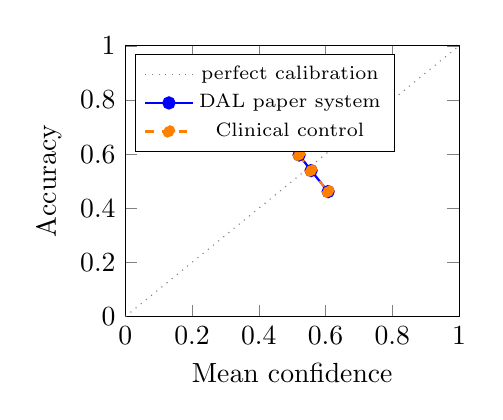
\begin{tikzpicture}
\begin{axis}[width=0.48\linewidth, xmin=0, xmax=1, ymin=0, ymax=1, xlabel={Mean confidence}, ylabel={Accuracy}, legend pos=north west, legend style={font=\scriptsize}]
\addplot[gray, dotted, domain=0:1] {x};
\addlegendentry{perfect calibration}
\addplot[blue, thick, mark=*] coordinates {(0.520667,0.596899) (0.556610,0.539106) (0.607671,0.461538)};
\addlegendentry{DAL paper system}
\addplot[orange, thick, dashed, mark=*] coordinates {(0.520667,0.596899) (0.556610,0.539106) (0.607671,0.461538)};
\addlegendentry{Clinical control}
\end{axis}
\end{tikzpicture}
\end{minipage}
\begin{minipage}{0.49\linewidth}\centering% Generated by tools/build_sg000024_manuscript_inputs.py from risk_coverage_source_data.json; do not edit.
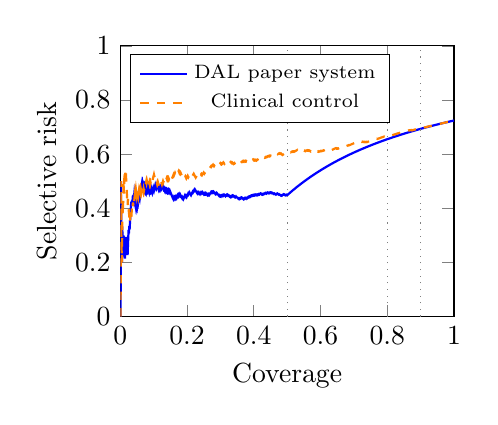
\begin{tikzpicture}
\begin{axis}[width=0.48\linewidth, xmin=0, xmax=1, ymin=0, ymax=1, xlabel={Coverage}, ylabel={Selective risk}, legend pos=north west, legend style={font=\scriptsize}]
\addplot[blue, thick] coordinates {(0.001000,0.000000) (0.002000,0.500000) (0.003000,0.333333) (0.004000,0.250000) (0.005000,0.200000) (0.006000,0.333333) (0.007000,0.285714) (0.008000,0.250000) (0.009000,0.222222) (0.010000,0.300000) (0.011000,0.272727) (0.012000,0.250000) (0.013000,0.230769) (0.014000,0.214286) (0.015000,0.266667) (0.016000,0.250000) (0.017000,0.294118) (0.018000,0.277778) (0.019000,0.263158) (0.020000,0.250000) (0.021000,0.238095) (0.022000,0.227273) (0.023000,0.260870) (0.024000,0.291667) (0.025000,0.320000) (0.026000,0.307692) (0.027000,0.333333) (0.028000,0.321429) (0.029000,0.344828) (0.030000,0.366667) (0.031000,0.387097) (0.032000,0.406250) (0.033000,0.424242) (0.034000,0.411765) (0.035000,0.428571) (0.036000,0.416667) (0.037000,0.432432) (0.038000,0.447368) (0.039000,0.435897) (0.040000,0.450000) (0.041000,0.439024) (0.042000,0.452381) (0.043000,0.441860) (0.044000,0.431818) (0.045000,0.422222) (0.046000,0.413043) (0.047000,0.425532) (0.048000,0.416667) (0.049000,0.408163) (0.050000,0.420000) (0.051000,0.411765) (0.052000,0.423077) (0.053000,0.433962) (0.054000,0.425926) (0.055000,0.436364) (0.056000,0.446429) (0.057000,0.456140) (0.058000,0.448276) (0.059000,0.440678) (0.060000,0.450000) (0.061000,0.459016) (0.062000,0.467742) (0.063000,0.476190) (0.064000,0.484375) (0.065000,0.492308) (0.066000,0.484848) (0.067000,0.492537) (0.068000,0.485294) (0.069000,0.478261) (0.070000,0.471429) (0.071000,0.478873) (0.072000,0.472222) (0.073000,0.479452) (0.074000,0.472973) (0.075000,0.466667) (0.076000,0.473684) (0.077000,0.467532) (0.078000,0.461538) (0.079000,0.468354) (0.080000,0.475000) (0.081000,0.469136) (0.082000,0.475610) (0.083000,0.469880) (0.084000,0.476190) (0.085000,0.470588) (0.086000,0.465116) (0.087000,0.459770) (0.088000,0.465909) (0.089000,0.471910) (0.090000,0.466667) (0.091000,0.472527) (0.092000,0.467391) (0.093000,0.473118) (0.094000,0.468085) (0.095000,0.463158) (0.096000,0.458333) (0.097000,0.463918) (0.098000,0.469388) (0.099000,0.474747) (0.100000,0.470000) (0.101000,0.465347) (0.102000,0.470588) (0.103000,0.475728) (0.104000,0.480769) (0.105000,0.485714) (0.106000,0.481132) (0.107000,0.476636) (0.108000,0.481481) (0.109000,0.477064) (0.110000,0.481818) (0.111000,0.486486) (0.112000,0.482143) (0.113000,0.477876) (0.114000,0.473684) (0.115000,0.469565) (0.116000,0.474138) (0.117000,0.470085) (0.118000,0.474576) (0.119000,0.478992) (0.120000,0.475000) (0.121000,0.471074) (0.122000,0.475410) (0.123000,0.479675) (0.124000,0.475806) (0.125000,0.480000) (0.126000,0.484127) (0.127000,0.480315) (0.128000,0.476562) (0.129000,0.472868) (0.130000,0.476923) (0.131000,0.473282) (0.132000,0.469697) (0.133000,0.466165) (0.134000,0.470149) (0.135000,0.466667) (0.136000,0.463235) (0.137000,0.467153) (0.138000,0.463768) (0.139000,0.467626) (0.140000,0.464286) (0.141000,0.460993) (0.142000,0.464789) (0.143000,0.461538) (0.144000,0.465278) (0.145000,0.462069) (0.146000,0.465753) (0.147000,0.462585) (0.148000,0.459459) (0.149000,0.463087) (0.150000,0.460000) (0.151000,0.456954) (0.152000,0.453947) (0.153000,0.450980) (0.154000,0.448052) (0.155000,0.445161) (0.156000,0.442308) (0.157000,0.439490) (0.158000,0.436709) (0.159000,0.433962) (0.160000,0.437500) (0.161000,0.440994) (0.162000,0.438272) (0.163000,0.435583) (0.164000,0.439024) (0.165000,0.436364) (0.166000,0.439759) (0.167000,0.443114) (0.168000,0.440476) (0.169000,0.437870) (0.170000,0.441176) (0.171000,0.444444) (0.172000,0.447674) (0.173000,0.445087) (0.174000,0.448276) (0.175000,0.445714) (0.176000,0.448864) (0.177000,0.451977) (0.178000,0.449438) (0.179000,0.446927) (0.180000,0.450000) (0.181000,0.447514) (0.182000,0.445055) (0.183000,0.442623) (0.184000,0.440217) (0.185000,0.437838) (0.186000,0.440860) (0.187000,0.438503) (0.188000,0.436170) (0.189000,0.433862) (0.190000,0.436842) (0.191000,0.439791) (0.192000,0.442708) (0.193000,0.445596) (0.194000,0.448454) (0.195000,0.446154) (0.196000,0.443878) (0.197000,0.441624) (0.198000,0.444444) (0.199000,0.442211) (0.200000,0.445000) (0.201000,0.447761) (0.202000,0.450495) (0.203000,0.453202) (0.204000,0.450980) (0.205000,0.453659) (0.206000,0.456311) (0.207000,0.458937) (0.208000,0.456731) (0.209000,0.454545) (0.210000,0.452381) (0.211000,0.450237) (0.212000,0.448113) (0.213000,0.450704) (0.214000,0.453271) (0.215000,0.455814) (0.216000,0.458333) (0.217000,0.460829) (0.218000,0.458716) (0.219000,0.461187) (0.220000,0.463636) (0.221000,0.466063) (0.222000,0.468468) (0.223000,0.466368) (0.224000,0.468750) (0.225000,0.466667) (0.226000,0.464602) (0.227000,0.462555) (0.228000,0.460526) (0.229000,0.458515) (0.230000,0.456522) (0.231000,0.454545) (0.232000,0.456897) (0.233000,0.459227) (0.234000,0.457265) (0.235000,0.455319) (0.236000,0.457627) (0.237000,0.455696) (0.238000,0.453782) (0.239000,0.451883) (0.240000,0.454167) (0.241000,0.456432) (0.242000,0.458678) (0.243000,0.456790) (0.244000,0.454918) (0.245000,0.457143) (0.246000,0.459350) (0.247000,0.457490) (0.248000,0.455645) (0.249000,0.453815) (0.250000,0.452000) (0.251000,0.454183) (0.252000,0.452381) (0.253000,0.454545) (0.254000,0.452756) (0.255000,0.454902) (0.256000,0.453125) (0.257000,0.455253) (0.258000,0.453488) (0.259000,0.451737) (0.260000,0.450000) (0.261000,0.448276) (0.262000,0.450382) (0.263000,0.452471) (0.264000,0.450758) (0.265000,0.449057) (0.266000,0.451128) (0.267000,0.449438) (0.268000,0.451493) (0.269000,0.453532) (0.270000,0.455556) (0.271000,0.457565) (0.272000,0.459559) (0.273000,0.457875) (0.274000,0.459854) (0.275000,0.458182) (0.276000,0.460145) (0.277000,0.458484) (0.278000,0.460432) (0.279000,0.458781) (0.280000,0.460714) (0.281000,0.459075) (0.282000,0.457447) (0.283000,0.455830) (0.284000,0.454225) (0.285000,0.452632) (0.286000,0.454545) (0.287000,0.452962) (0.288000,0.454861) (0.289000,0.456747) (0.290000,0.455172) (0.291000,0.453608) (0.292000,0.452055) (0.293000,0.450512) (0.294000,0.448980) (0.295000,0.447458) (0.296000,0.445946) (0.297000,0.447811) (0.298000,0.446309) (0.299000,0.444816) (0.300000,0.446667) (0.301000,0.445183) (0.302000,0.443709) (0.303000,0.445545) (0.304000,0.447368) (0.305000,0.445902) (0.306000,0.447712) (0.307000,0.446254) (0.308000,0.448052) (0.309000,0.446602) (0.310000,0.448387) (0.311000,0.450161) (0.312000,0.448718) (0.313000,0.447284) (0.314000,0.445860) (0.315000,0.444444) (0.316000,0.446203) (0.317000,0.447950) (0.318000,0.449686) (0.319000,0.448276) (0.320000,0.446875) (0.321000,0.448598) (0.322000,0.450311) (0.323000,0.448916) (0.324000,0.447531) (0.325000,0.446154) (0.326000,0.444785) (0.327000,0.443425) (0.328000,0.445122) (0.329000,0.443769) (0.330000,0.442424) (0.331000,0.441088) (0.332000,0.442771) (0.333000,0.444444) (0.334000,0.443114) (0.335000,0.444776) (0.336000,0.446429) (0.337000,0.445104) (0.338000,0.446746) (0.339000,0.445428) (0.340000,0.444118) (0.341000,0.442815) (0.342000,0.441520) (0.343000,0.443149) (0.344000,0.441860) (0.345000,0.440580) (0.346000,0.442197) (0.347000,0.443804) (0.348000,0.442529) (0.349000,0.441261) (0.350000,0.440000) (0.351000,0.438746) (0.352000,0.437500) (0.353000,0.436261) (0.354000,0.435028) (0.355000,0.436620) (0.356000,0.435393) (0.357000,0.434174) (0.358000,0.435754) (0.359000,0.437326) (0.360000,0.436111) (0.361000,0.437673) (0.362000,0.439227) (0.363000,0.438017) (0.364000,0.439560) (0.365000,0.438356) (0.366000,0.437158) (0.367000,0.435967) (0.368000,0.434783) (0.369000,0.433604) (0.370000,0.435135) (0.371000,0.433962) (0.372000,0.435484) (0.373000,0.436997) (0.374000,0.438503) (0.375000,0.437333) (0.376000,0.436170) (0.377000,0.435013) (0.378000,0.436508) (0.379000,0.437995) (0.380000,0.436842) (0.381000,0.438320) (0.382000,0.439791) (0.383000,0.441253) (0.384000,0.440104) (0.385000,0.441558) (0.386000,0.443005) (0.387000,0.441860) (0.388000,0.443299) (0.389000,0.442159) (0.390000,0.443590) (0.391000,0.445013) (0.392000,0.446429) (0.393000,0.445293) (0.394000,0.446701) (0.395000,0.445570) (0.396000,0.446970) (0.397000,0.448363) (0.398000,0.447236) (0.399000,0.448622) (0.400000,0.447500) (0.401000,0.448878) (0.402000,0.447761) (0.403000,0.449132) (0.404000,0.450495) (0.405000,0.449383) (0.406000,0.448276) (0.407000,0.449631) (0.408000,0.448529) (0.409000,0.449878) (0.410000,0.448780) (0.411000,0.450122) (0.412000,0.449029) (0.413000,0.450363) (0.414000,0.451691) (0.415000,0.450602) (0.416000,0.451923) (0.417000,0.450839) (0.418000,0.452153) (0.419000,0.453461) (0.420000,0.454762) (0.421000,0.453682) (0.422000,0.452607) (0.423000,0.451537) (0.424000,0.452830) (0.425000,0.451765) (0.426000,0.450704) (0.427000,0.451991) (0.428000,0.450935) (0.429000,0.452214) (0.430000,0.453488) (0.431000,0.452436) (0.432000,0.453704) (0.433000,0.454965) (0.434000,0.456221) (0.435000,0.455172) (0.436000,0.456422) (0.437000,0.455378) (0.438000,0.454338) (0.439000,0.455581) (0.440000,0.456818) (0.441000,0.458050) (0.442000,0.457014) (0.443000,0.455982) (0.444000,0.457207) (0.445000,0.456180) (0.446000,0.455157) (0.447000,0.456376) (0.448000,0.457589) (0.449000,0.458797) (0.450000,0.457778) (0.451000,0.456763) (0.452000,0.457965) (0.453000,0.456954) (0.454000,0.455947) (0.455000,0.457143) (0.456000,0.456140) (0.457000,0.455142) (0.458000,0.454148) (0.459000,0.453159) (0.460000,0.454348) (0.461000,0.453362) (0.462000,0.454545) (0.463000,0.453564) (0.464000,0.452586) (0.465000,0.451613) (0.466000,0.450644) (0.467000,0.451820) (0.468000,0.452991) (0.469000,0.452026) (0.470000,0.453191) (0.471000,0.454352) (0.472000,0.453390) (0.473000,0.452431) (0.474000,0.451477) (0.475000,0.450526) (0.476000,0.451681) (0.477000,0.450734) (0.478000,0.449791) (0.479000,0.448852) (0.480000,0.447917) (0.481000,0.446985) (0.482000,0.448133) (0.483000,0.447205) (0.484000,0.446281) (0.485000,0.447423) (0.486000,0.448560) (0.487000,0.449692) (0.488000,0.450820) (0.489000,0.451943) (0.490000,0.451020) (0.491000,0.450102) (0.492000,0.449187) (0.493000,0.450304) (0.494000,0.449393) (0.495000,0.448485) (0.496000,0.447581) (0.497000,0.448692) (0.498000,0.449799) (0.499000,0.448898) (0.500000,0.448000) (0.501000,0.449102) (0.502000,0.450199) (0.503000,0.451292) (0.504000,0.452381) (0.505000,0.453465) (0.506000,0.454545) (0.507000,0.455621) (0.508000,0.456693) (0.509000,0.457760) (0.510000,0.458824) (0.511000,0.459883) (0.512000,0.460938) (0.513000,0.461988) (0.514000,0.463035) (0.515000,0.464078) (0.516000,0.465116) (0.517000,0.466151) (0.518000,0.467181) (0.519000,0.468208) (0.520000,0.469231) (0.521000,0.470250) (0.522000,0.471264) (0.523000,0.472275) (0.524000,0.473282) (0.525000,0.474286) (0.526000,0.475285) (0.527000,0.476281) (0.528000,0.477273) (0.529000,0.478261) (0.530000,0.479245) (0.531000,0.480226) (0.532000,0.481203) (0.533000,0.482176) (0.534000,0.483146) (0.535000,0.484112) (0.536000,0.485075) (0.537000,0.486034) (0.538000,0.486989) (0.539000,0.487941) (0.540000,0.488889) (0.541000,0.489834) (0.542000,0.490775) (0.543000,0.491713) (0.544000,0.492647) (0.545000,0.493578) (0.546000,0.494505) (0.547000,0.495430) (0.548000,0.496350) (0.549000,0.497268) (0.550000,0.498182) (0.551000,0.499093) (0.552000,0.500000) (0.553000,0.500904) (0.554000,0.501805) (0.555000,0.502703) (0.556000,0.503597) (0.557000,0.504488) (0.558000,0.505376) (0.559000,0.506261) (0.560000,0.507143) (0.561000,0.508021) (0.562000,0.508897) (0.563000,0.509769) (0.564000,0.510638) (0.565000,0.511504) (0.566000,0.512367) (0.567000,0.513228) (0.568000,0.514085) (0.569000,0.514938) (0.570000,0.515789) (0.571000,0.516637) (0.572000,0.517483) (0.573000,0.518325) (0.574000,0.519164) (0.575000,0.520000) (0.576000,0.520833) (0.577000,0.521664) (0.578000,0.522491) (0.579000,0.523316) (0.580000,0.524138) (0.581000,0.524957) (0.582000,0.525773) (0.583000,0.526587) (0.584000,0.527397) (0.585000,0.528205) (0.586000,0.529010) (0.587000,0.529813) (0.588000,0.530612) (0.589000,0.531409) (0.590000,0.532203) (0.591000,0.532995) (0.592000,0.533784) (0.593000,0.534570) (0.594000,0.535354) (0.595000,0.536134) (0.596000,0.536913) (0.597000,0.537688) (0.598000,0.538462) (0.599000,0.539232) (0.600000,0.540000) (0.601000,0.540765) (0.602000,0.541528) (0.603000,0.542289) (0.604000,0.543046) (0.605000,0.543802) (0.606000,0.544554) (0.607000,0.545305) (0.608000,0.546053) (0.609000,0.546798) (0.610000,0.547541) (0.611000,0.548282) (0.612000,0.549020) (0.613000,0.549755) (0.614000,0.550489) (0.615000,0.551220) (0.616000,0.551948) (0.617000,0.552674) (0.618000,0.553398) (0.619000,0.554120) (0.620000,0.554839) (0.621000,0.555556) (0.622000,0.556270) (0.623000,0.556982) (0.624000,0.557692) (0.625000,0.558400) (0.626000,0.559105) (0.627000,0.559809) (0.628000,0.560510) (0.629000,0.561208) (0.630000,0.561905) (0.631000,0.562599) (0.632000,0.563291) (0.633000,0.563981) (0.634000,0.564669) (0.635000,0.565354) (0.636000,0.566038) (0.637000,0.566719) (0.638000,0.567398) (0.639000,0.568075) (0.640000,0.568750) (0.641000,0.569423) (0.642000,0.570093) (0.643000,0.570762) (0.644000,0.571429) (0.645000,0.572093) (0.646000,0.572755) (0.647000,0.573416) (0.648000,0.574074) (0.649000,0.574730) (0.650000,0.575385) (0.651000,0.576037) (0.652000,0.576687) (0.653000,0.577335) (0.654000,0.577982) (0.655000,0.578626) (0.656000,0.579268) (0.657000,0.579909) (0.658000,0.580547) (0.659000,0.581184) (0.660000,0.581818) (0.661000,0.582451) (0.662000,0.583082) (0.663000,0.583710) (0.664000,0.584337) (0.665000,0.584962) (0.666000,0.585586) (0.667000,0.586207) (0.668000,0.586826) (0.669000,0.587444) (0.670000,0.588060) (0.671000,0.588674) (0.672000,0.589286) (0.673000,0.589896) (0.674000,0.590504) (0.675000,0.591111) (0.676000,0.591716) (0.677000,0.592319) (0.678000,0.592920) (0.679000,0.593520) (0.680000,0.594118) (0.681000,0.594714) (0.682000,0.595308) (0.683000,0.595900) (0.684000,0.596491) (0.685000,0.597080) (0.686000,0.597668) (0.687000,0.598253) (0.688000,0.598837) (0.689000,0.599419) (0.690000,0.600000) (0.691000,0.600579) (0.692000,0.601156) (0.693000,0.601732) (0.694000,0.602305) (0.695000,0.602878) (0.696000,0.603448) (0.697000,0.604017) (0.698000,0.604585) (0.699000,0.605150) (0.700000,0.605714) (0.701000,0.606277) (0.702000,0.606838) (0.703000,0.607397) (0.704000,0.607955) (0.705000,0.608511) (0.706000,0.609065) (0.707000,0.609618) (0.708000,0.610169) (0.709000,0.610719) (0.710000,0.611268) (0.711000,0.611814) (0.712000,0.612360) (0.713000,0.612903) (0.714000,0.613445) (0.715000,0.613986) (0.716000,0.614525) (0.717000,0.615063) (0.718000,0.615599) (0.719000,0.616134) (0.720000,0.616667) (0.721000,0.617198) (0.722000,0.617729) (0.723000,0.618257) (0.724000,0.618785) (0.725000,0.619310) (0.726000,0.619835) (0.727000,0.620358) (0.728000,0.620879) (0.729000,0.621399) (0.730000,0.621918) (0.731000,0.622435) (0.732000,0.622951) (0.733000,0.623465) (0.734000,0.623978) (0.735000,0.624490) (0.736000,0.625000) (0.737000,0.625509) (0.738000,0.626016) (0.739000,0.626522) (0.740000,0.627027) (0.741000,0.627530) (0.742000,0.628032) (0.743000,0.628533) (0.744000,0.629032) (0.745000,0.629530) (0.746000,0.630027) (0.747000,0.630522) (0.748000,0.631016) (0.749000,0.631509) (0.750000,0.632000) (0.751000,0.632490) (0.752000,0.632979) (0.753000,0.633466) (0.754000,0.633952) (0.755000,0.634437) (0.756000,0.634921) (0.757000,0.635403) (0.758000,0.635884) (0.759000,0.636364) (0.760000,0.636842) (0.761000,0.637319) (0.762000,0.637795) (0.763000,0.638270) (0.764000,0.638743) (0.765000,0.639216) (0.766000,0.639687) (0.767000,0.640156) (0.768000,0.640625) (0.769000,0.641092) (0.770000,0.641558) (0.771000,0.642023) (0.772000,0.642487) (0.773000,0.642950) (0.774000,0.643411) (0.775000,0.643871) (0.776000,0.644330) (0.777000,0.644788) (0.778000,0.645244) (0.779000,0.645700) (0.780000,0.646154) (0.781000,0.646607) (0.782000,0.647059) (0.783000,0.647510) (0.784000,0.647959) (0.785000,0.648408) (0.786000,0.648855) (0.787000,0.649301) (0.788000,0.649746) (0.789000,0.650190) (0.790000,0.650633) (0.791000,0.651075) (0.792000,0.651515) (0.793000,0.651955) (0.794000,0.652393) (0.795000,0.652830) (0.796000,0.653266) (0.797000,0.653701) (0.798000,0.654135) (0.799000,0.654568) (0.800000,0.655000) (0.801000,0.655431) (0.802000,0.655860) (0.803000,0.656289) (0.804000,0.656716) (0.805000,0.657143) (0.806000,0.657568) (0.807000,0.657993) (0.808000,0.658416) (0.809000,0.658838) (0.810000,0.659259) (0.811000,0.659679) (0.812000,0.660099) (0.813000,0.660517) (0.814000,0.660934) (0.815000,0.661350) (0.816000,0.661765) (0.817000,0.662179) (0.818000,0.662592) (0.819000,0.663004) (0.820000,0.663415) (0.821000,0.663825) (0.822000,0.664234) (0.823000,0.664642) (0.824000,0.665049) (0.825000,0.665455) (0.826000,0.665860) (0.827000,0.666264) (0.828000,0.666667) (0.829000,0.667069) (0.830000,0.667470) (0.831000,0.667870) (0.832000,0.668269) (0.833000,0.668667) (0.834000,0.669065) (0.835000,0.669461) (0.836000,0.669856) (0.837000,0.670251) (0.838000,0.670644) (0.839000,0.671037) (0.840000,0.671429) (0.841000,0.671819) (0.842000,0.672209) (0.843000,0.672598) (0.844000,0.672986) (0.845000,0.673373) (0.846000,0.673759) (0.847000,0.674144) (0.848000,0.674528) (0.849000,0.674912) (0.850000,0.675294) (0.851000,0.675676) (0.852000,0.676056) (0.853000,0.676436) (0.854000,0.676815) (0.855000,0.677193) (0.856000,0.677570) (0.857000,0.677946) (0.858000,0.678322) (0.859000,0.678696) (0.860000,0.679070) (0.861000,0.679443) (0.862000,0.679814) (0.863000,0.680185) (0.864000,0.680556) (0.865000,0.680925) (0.866000,0.681293) (0.867000,0.681661) (0.868000,0.682028) (0.869000,0.682394) (0.870000,0.682759) (0.871000,0.683123) (0.872000,0.683486) (0.873000,0.683849) (0.874000,0.684211) (0.875000,0.684571) (0.876000,0.684932) (0.877000,0.685291) (0.878000,0.685649) (0.879000,0.686007) (0.880000,0.686364) (0.881000,0.686720) (0.882000,0.687075) (0.883000,0.687429) (0.884000,0.687783) (0.885000,0.688136) (0.886000,0.688488) (0.887000,0.688839) (0.888000,0.689189) (0.889000,0.689539) (0.890000,0.689888) (0.891000,0.690236) (0.892000,0.690583) (0.893000,0.690929) (0.894000,0.691275) (0.895000,0.691620) (0.896000,0.691964) (0.897000,0.692308) (0.898000,0.692650) (0.899000,0.692992) (0.900000,0.693333) (0.901000,0.693674) (0.902000,0.694013) (0.903000,0.694352) (0.904000,0.694690) (0.905000,0.695028) (0.906000,0.695364) (0.907000,0.695700) (0.908000,0.696035) (0.909000,0.696370) (0.910000,0.696703) (0.911000,0.697036) (0.912000,0.697368) (0.913000,0.697700) (0.914000,0.698031) (0.915000,0.698361) (0.916000,0.698690) (0.917000,0.699019) (0.918000,0.699346) (0.919000,0.699674) (0.920000,0.700000) (0.921000,0.700326) (0.922000,0.700651) (0.923000,0.700975) (0.924000,0.701299) (0.925000,0.701622) (0.926000,0.701944) (0.927000,0.702265) (0.928000,0.702586) (0.929000,0.702906) (0.930000,0.703226) (0.931000,0.703545) (0.932000,0.703863) (0.933000,0.704180) (0.934000,0.704497) (0.935000,0.704813) (0.936000,0.705128) (0.937000,0.705443) (0.938000,0.705757) (0.939000,0.706070) (0.940000,0.706383) (0.941000,0.706695) (0.942000,0.707006) (0.943000,0.707317) (0.944000,0.707627) (0.945000,0.707937) (0.946000,0.708245) (0.947000,0.708553) (0.948000,0.708861) (0.949000,0.709168) (0.950000,0.709474) (0.951000,0.709779) (0.952000,0.710084) (0.953000,0.710388) (0.954000,0.710692) (0.955000,0.710995) (0.956000,0.711297) (0.957000,0.711599) (0.958000,0.711900) (0.959000,0.712200) (0.960000,0.712500) (0.961000,0.712799) (0.962000,0.713098) (0.963000,0.713396) (0.964000,0.713693) (0.965000,0.713990) (0.966000,0.714286) (0.967000,0.714581) (0.968000,0.714876) (0.969000,0.715170) (0.970000,0.715464) (0.971000,0.715757) (0.972000,0.716049) (0.973000,0.716341) (0.974000,0.716632) (0.975000,0.716923) (0.976000,0.717213) (0.977000,0.717503) (0.978000,0.717791) (0.979000,0.718080) (0.980000,0.718367) (0.981000,0.718654) (0.982000,0.718941) (0.983000,0.719227) (0.984000,0.719512) (0.985000,0.719797) (0.986000,0.720081) (0.987000,0.720365) (0.988000,0.720648) (0.989000,0.720930) (0.990000,0.721212) (0.991000,0.721493) (0.992000,0.721774) (0.993000,0.722054) (0.994000,0.722334) (0.995000,0.722613) (0.996000,0.722892) (0.997000,0.723170) (0.998000,0.723447) (0.999000,0.723724) (1.000000,0.724000)};
\addlegendentry{DAL paper system}
\addplot[orange, thick, dashed] coordinates {(0.001000,0.000000) (0.002000,0.500000) (0.003000,0.333333) (0.004000,0.250000) (0.005000,0.200000) (0.006000,0.333333) (0.007000,0.428571) (0.008000,0.375000) (0.009000,0.444444) (0.010000,0.500000) (0.011000,0.454545) (0.012000,0.500000) (0.013000,0.538462) (0.014000,0.500000) (0.015000,0.533333) (0.016000,0.500000) (0.017000,0.529412) (0.018000,0.500000) (0.019000,0.473684) (0.020000,0.450000) (0.021000,0.428571) (0.022000,0.409091) (0.023000,0.434783) (0.024000,0.416667) (0.025000,0.400000) (0.026000,0.384615) (0.027000,0.370370) (0.028000,0.357143) (0.029000,0.344828) (0.030000,0.366667) (0.031000,0.387097) (0.032000,0.375000) (0.033000,0.363636) (0.034000,0.382353) (0.035000,0.400000) (0.036000,0.388889) (0.037000,0.405405) (0.038000,0.421053) (0.039000,0.410256) (0.040000,0.425000) (0.041000,0.414634) (0.042000,0.428571) (0.043000,0.441860) (0.044000,0.454545) (0.045000,0.444444) (0.046000,0.456522) (0.047000,0.468085) (0.048000,0.458333) (0.049000,0.448980) (0.050000,0.460000) (0.051000,0.450980) (0.052000,0.442308) (0.053000,0.452830) (0.054000,0.444444) (0.055000,0.454545) (0.056000,0.464286) (0.057000,0.456140) (0.058000,0.448276) (0.059000,0.457627) (0.060000,0.466667) (0.061000,0.459016) (0.062000,0.467742) (0.063000,0.460317) (0.064000,0.468750) (0.065000,0.476923) (0.066000,0.484848) (0.067000,0.477612) (0.068000,0.470588) (0.069000,0.463768) (0.070000,0.471429) (0.071000,0.464789) (0.072000,0.472222) (0.073000,0.465753) (0.074000,0.472973) (0.075000,0.480000) (0.076000,0.486842) (0.077000,0.493506) (0.078000,0.500000) (0.079000,0.493671) (0.080000,0.500000) (0.081000,0.493827) (0.082000,0.500000) (0.083000,0.493976) (0.084000,0.488095) (0.085000,0.494118) (0.086000,0.488372) (0.087000,0.494253) (0.088000,0.488636) (0.089000,0.494382) (0.090000,0.488889) (0.091000,0.494505) (0.092000,0.489130) (0.093000,0.494624) (0.094000,0.500000) (0.095000,0.505263) (0.096000,0.500000) (0.097000,0.505155) (0.098000,0.510204) (0.099000,0.515152) (0.100000,0.520000) (0.101000,0.524752) (0.102000,0.519608) (0.103000,0.514563) (0.104000,0.509615) (0.105000,0.504762) (0.106000,0.500000) (0.107000,0.495327) (0.108000,0.490741) (0.109000,0.495413) (0.110000,0.490909) (0.111000,0.495495) (0.112000,0.491071) (0.113000,0.495575) (0.114000,0.491228) (0.115000,0.486957) (0.116000,0.482759) (0.117000,0.487179) (0.118000,0.491525) (0.119000,0.495798) (0.120000,0.491667) (0.121000,0.495868) (0.122000,0.500000) (0.123000,0.495935) (0.124000,0.491935) (0.125000,0.488000) (0.126000,0.492063) (0.127000,0.496063) (0.128000,0.500000) (0.129000,0.496124) (0.130000,0.500000) (0.131000,0.503817) (0.132000,0.507576) (0.133000,0.511278) (0.134000,0.507463) (0.135000,0.511111) (0.136000,0.507353) (0.137000,0.510949) (0.138000,0.507246) (0.139000,0.510791) (0.140000,0.507143) (0.141000,0.510638) (0.142000,0.507042) (0.143000,0.510490) (0.144000,0.506944) (0.145000,0.510345) (0.146000,0.506849) (0.147000,0.510204) (0.148000,0.506757) (0.149000,0.503356) (0.150000,0.506667) (0.151000,0.509934) (0.152000,0.506579) (0.153000,0.509804) (0.154000,0.506494) (0.155000,0.509677) (0.156000,0.512821) (0.157000,0.515924) (0.158000,0.518987) (0.159000,0.522013) (0.160000,0.525000) (0.161000,0.521739) (0.162000,0.524691) (0.163000,0.527607) (0.164000,0.530488) (0.165000,0.527273) (0.166000,0.524096) (0.167000,0.520958) (0.168000,0.523810) (0.169000,0.526627) (0.170000,0.529412) (0.171000,0.532164) (0.172000,0.529070) (0.173000,0.531792) (0.174000,0.534483) (0.175000,0.537143) (0.176000,0.534091) (0.177000,0.531073) (0.178000,0.533708) (0.179000,0.530726) (0.180000,0.527778) (0.181000,0.530387) (0.182000,0.527473) (0.183000,0.524590) (0.184000,0.521739) (0.185000,0.518919) (0.186000,0.521505) (0.187000,0.518717) (0.188000,0.521277) (0.189000,0.523810) (0.190000,0.521053) (0.191000,0.518325) (0.192000,0.515625) (0.193000,0.518135) (0.194000,0.515464) (0.195000,0.517949) (0.196000,0.515306) (0.197000,0.512690) (0.198000,0.510101) (0.199000,0.512563) (0.200000,0.515000) (0.201000,0.517413) (0.202000,0.519802) (0.203000,0.517241) (0.204000,0.514706) (0.205000,0.517073) (0.206000,0.519417) (0.207000,0.516908) (0.208000,0.514423) (0.209000,0.516746) (0.210000,0.519048) (0.211000,0.521327) (0.212000,0.523585) (0.213000,0.521127) (0.214000,0.518692) (0.215000,0.520930) (0.216000,0.518519) (0.217000,0.520737) (0.218000,0.522936) (0.219000,0.525114) (0.220000,0.527273) (0.221000,0.524887) (0.222000,0.522523) (0.223000,0.520179) (0.224000,0.517857) (0.225000,0.515556) (0.226000,0.513274) (0.227000,0.515419) (0.228000,0.517544) (0.229000,0.519651) (0.230000,0.521739) (0.231000,0.523810) (0.232000,0.521552) (0.233000,0.523605) (0.234000,0.525641) (0.235000,0.523404) (0.236000,0.521186) (0.237000,0.518987) (0.238000,0.521008) (0.239000,0.523013) (0.240000,0.525000) (0.241000,0.526971) (0.242000,0.524793) (0.243000,0.526749) (0.244000,0.524590) (0.245000,0.522449) (0.246000,0.524390) (0.247000,0.526316) (0.248000,0.528226) (0.249000,0.530120) (0.250000,0.532000) (0.251000,0.529880) (0.252000,0.527778) (0.253000,0.529644) (0.254000,0.531496) (0.255000,0.533333) (0.256000,0.531250) (0.257000,0.533074) (0.258000,0.534884) (0.259000,0.536680) (0.260000,0.538462) (0.261000,0.540230) (0.262000,0.541985) (0.263000,0.543726) (0.264000,0.545455) (0.265000,0.543396) (0.266000,0.545113) (0.267000,0.546816) (0.268000,0.548507) (0.269000,0.550186) (0.270000,0.551852) (0.271000,0.553506) (0.272000,0.555147) (0.273000,0.553114) (0.274000,0.554745) (0.275000,0.556364) (0.276000,0.557971) (0.277000,0.559567) (0.278000,0.561151) (0.279000,0.559140) (0.280000,0.557143) (0.281000,0.555160) (0.282000,0.556738) (0.283000,0.554770) (0.284000,0.556338) (0.285000,0.557895) (0.286000,0.559441) (0.287000,0.557491) (0.288000,0.559028) (0.289000,0.557093) (0.290000,0.558621) (0.291000,0.560137) (0.292000,0.558219) (0.293000,0.559727) (0.294000,0.557823) (0.295000,0.559322) (0.296000,0.560811) (0.297000,0.562290) (0.298000,0.563758) (0.299000,0.565217) (0.300000,0.566667) (0.301000,0.564784) (0.302000,0.562914) (0.303000,0.564356) (0.304000,0.562500) (0.305000,0.563934) (0.306000,0.565359) (0.307000,0.566775) (0.308000,0.568182) (0.309000,0.569579) (0.310000,0.567742) (0.311000,0.565916) (0.312000,0.564103) (0.313000,0.565495) (0.314000,0.566879) (0.315000,0.565079) (0.316000,0.566456) (0.317000,0.564669) (0.318000,0.566038) (0.319000,0.567398) (0.320000,0.568750) (0.321000,0.570093) (0.322000,0.568323) (0.323000,0.566563) (0.324000,0.567901) (0.325000,0.566154) (0.326000,0.567485) (0.327000,0.565749) (0.328000,0.567073) (0.329000,0.568389) (0.330000,0.569697) (0.331000,0.570997) (0.332000,0.569277) (0.333000,0.567568) (0.334000,0.568862) (0.335000,0.567164) (0.336000,0.568452) (0.337000,0.566766) (0.338000,0.565089) (0.339000,0.563422) (0.340000,0.564706) (0.341000,0.565982) (0.342000,0.567251) (0.343000,0.565598) (0.344000,0.566860) (0.345000,0.568116) (0.346000,0.566474) (0.347000,0.567723) (0.348000,0.568966) (0.349000,0.570201) (0.350000,0.571429) (0.351000,0.569801) (0.352000,0.568182) (0.353000,0.566572) (0.354000,0.567797) (0.355000,0.569014) (0.356000,0.570225) (0.357000,0.571429) (0.358000,0.569832) (0.359000,0.571031) (0.360000,0.569444) (0.361000,0.567867) (0.362000,0.569061) (0.363000,0.570248) (0.364000,0.571429) (0.365000,0.572603) (0.366000,0.573770) (0.367000,0.572207) (0.368000,0.573370) (0.369000,0.574526) (0.370000,0.572973) (0.371000,0.571429) (0.372000,0.572581) (0.373000,0.573727) (0.374000,0.574866) (0.375000,0.573333) (0.376000,0.574468) (0.377000,0.572944) (0.378000,0.574074) (0.379000,0.572559) (0.380000,0.571053) (0.381000,0.572178) (0.382000,0.573298) (0.383000,0.574413) (0.384000,0.575521) (0.385000,0.576623) (0.386000,0.577720) (0.387000,0.576227) (0.388000,0.574742) (0.389000,0.575835) (0.390000,0.576923) (0.391000,0.578005) (0.392000,0.576531) (0.393000,0.577608) (0.394000,0.578680) (0.395000,0.577215) (0.396000,0.578283) (0.397000,0.579345) (0.398000,0.580402) (0.399000,0.578947) (0.400000,0.577500) (0.401000,0.578554) (0.402000,0.577114) (0.403000,0.578164) (0.404000,0.576733) (0.405000,0.577778) (0.406000,0.578818) (0.407000,0.577396) (0.408000,0.575980) (0.409000,0.577017) (0.410000,0.578049) (0.411000,0.579075) (0.412000,0.580097) (0.413000,0.581114) (0.414000,0.582126) (0.415000,0.583133) (0.416000,0.584135) (0.417000,0.582734) (0.418000,0.583732) (0.419000,0.584726) (0.420000,0.585714) (0.421000,0.586698) (0.422000,0.587678) (0.423000,0.588652) (0.424000,0.589623) (0.425000,0.590588) (0.426000,0.589202) (0.427000,0.590164) (0.428000,0.588785) (0.429000,0.587413) (0.430000,0.586047) (0.431000,0.587007) (0.432000,0.587963) (0.433000,0.586605) (0.434000,0.587558) (0.435000,0.588506) (0.436000,0.589450) (0.437000,0.588101) (0.438000,0.589041) (0.439000,0.589977) (0.440000,0.590909) (0.441000,0.591837) (0.442000,0.590498) (0.443000,0.591422) (0.444000,0.592342) (0.445000,0.593258) (0.446000,0.594170) (0.447000,0.592841) (0.448000,0.591518) (0.449000,0.592428) (0.450000,0.593333) (0.451000,0.594235) (0.452000,0.592920) (0.453000,0.593819) (0.454000,0.594714) (0.455000,0.593407) (0.456000,0.594298) (0.457000,0.595186) (0.458000,0.596070) (0.459000,0.596950) (0.460000,0.597826) (0.461000,0.598698) (0.462000,0.599567) (0.463000,0.598272) (0.464000,0.599138) (0.465000,0.600000) (0.466000,0.600858) (0.467000,0.599572) (0.468000,0.600427) (0.469000,0.601279) (0.470000,0.600000) (0.471000,0.600849) (0.472000,0.599576) (0.473000,0.600423) (0.474000,0.601266) (0.475000,0.602105) (0.476000,0.602941) (0.477000,0.601677) (0.478000,0.602510) (0.479000,0.603340) (0.480000,0.602083) (0.481000,0.600832) (0.482000,0.601660) (0.483000,0.600414) (0.484000,0.599174) (0.485000,0.597938) (0.486000,0.596708) (0.487000,0.597536) (0.488000,0.598361) (0.489000,0.599182) (0.490000,0.600000) (0.491000,0.600815) (0.492000,0.601626) (0.493000,0.602434) (0.494000,0.601215) (0.495000,0.602020) (0.496000,0.602823) (0.497000,0.601610) (0.498000,0.602410) (0.499000,0.603206) (0.500000,0.604000) (0.501000,0.602794) (0.502000,0.603586) (0.503000,0.604374) (0.504000,0.605159) (0.505000,0.603960) (0.506000,0.604743) (0.507000,0.605523) (0.508000,0.606299) (0.509000,0.607073) (0.510000,0.607843) (0.511000,0.606654) (0.512000,0.607422) (0.513000,0.608187) (0.514000,0.608949) (0.515000,0.609709) (0.516000,0.608527) (0.517000,0.609284) (0.518000,0.610039) (0.519000,0.608863) (0.520000,0.609615) (0.521000,0.610365) (0.522000,0.609195) (0.523000,0.609943) (0.524000,0.610687) (0.525000,0.611429) (0.526000,0.612167) (0.527000,0.612903) (0.528000,0.613636) (0.529000,0.614367) (0.530000,0.615094) (0.531000,0.615819) (0.532000,0.614662) (0.533000,0.615385) (0.534000,0.616105) (0.535000,0.614953) (0.536000,0.613806) (0.537000,0.614525) (0.538000,0.615242) (0.539000,0.614100) (0.540000,0.612963) (0.541000,0.611830) (0.542000,0.610701) (0.543000,0.611418) (0.544000,0.612132) (0.545000,0.612844) (0.546000,0.613553) (0.547000,0.614260) (0.548000,0.614964) (0.549000,0.613843) (0.550000,0.614545) (0.551000,0.613430) (0.552000,0.612319) (0.553000,0.613020) (0.554000,0.611913) (0.555000,0.610811) (0.556000,0.611511) (0.557000,0.612208) (0.558000,0.612903) (0.559000,0.613596) (0.560000,0.614286) (0.561000,0.613191) (0.562000,0.613879) (0.563000,0.612789) (0.564000,0.613475) (0.565000,0.612389) (0.566000,0.613074) (0.567000,0.611993) (0.568000,0.612676) (0.569000,0.611599) (0.570000,0.610526) (0.571000,0.609457) (0.572000,0.610140) (0.573000,0.610820) (0.574000,0.611498) (0.575000,0.610435) (0.576000,0.609375) (0.577000,0.610052) (0.578000,0.610727) (0.579000,0.611399) (0.580000,0.612069) (0.581000,0.611015) (0.582000,0.611684) (0.583000,0.612350) (0.584000,0.611301) (0.585000,0.611966) (0.586000,0.612628) (0.587000,0.611584) (0.588000,0.612245) (0.589000,0.611205) (0.590000,0.610169) (0.591000,0.610829) (0.592000,0.609797) (0.593000,0.610455) (0.594000,0.609428) (0.595000,0.608403) (0.596000,0.609060) (0.597000,0.609715) (0.598000,0.610368) (0.599000,0.611018) (0.600000,0.611667) (0.601000,0.610649) (0.602000,0.611296) (0.603000,0.611940) (0.604000,0.610927) (0.605000,0.611570) (0.606000,0.612211) (0.607000,0.612850) (0.608000,0.613487) (0.609000,0.614122) (0.610000,0.613115) (0.611000,0.613748) (0.612000,0.614379) (0.613000,0.615008) (0.614000,0.615635) (0.615000,0.616260) (0.616000,0.616883) (0.617000,0.617504) (0.618000,0.616505) (0.619000,0.617124) (0.620000,0.617742) (0.621000,0.616747) (0.622000,0.617363) (0.623000,0.617978) (0.624000,0.616987) (0.625000,0.617600) (0.626000,0.616613) (0.627000,0.617225) (0.628000,0.617834) (0.629000,0.616852) (0.630000,0.615873) (0.631000,0.614897) (0.632000,0.615506) (0.633000,0.616114) (0.634000,0.615142) (0.635000,0.615748) (0.636000,0.616352) (0.637000,0.616954) (0.638000,0.617555) (0.639000,0.618153) (0.640000,0.618750) (0.641000,0.619345) (0.642000,0.619938) (0.643000,0.620529) (0.644000,0.621118) (0.645000,0.621705) (0.646000,0.622291) (0.647000,0.621329) (0.648000,0.620370) (0.649000,0.620955) (0.650000,0.620000) (0.651000,0.620584) (0.652000,0.621166) (0.653000,0.620214) (0.654000,0.620795) (0.655000,0.621374) (0.656000,0.621951) (0.657000,0.622527) (0.658000,0.623100) (0.659000,0.623672) (0.660000,0.624242) (0.661000,0.624811) (0.662000,0.625378) (0.663000,0.624434) (0.664000,0.625000) (0.665000,0.625564) (0.666000,0.624625) (0.667000,0.625187) (0.668000,0.625749) (0.669000,0.626308) (0.670000,0.625373) (0.671000,0.625931) (0.672000,0.626488) (0.673000,0.627043) (0.674000,0.627596) (0.675000,0.628148) (0.676000,0.628698) (0.677000,0.629247) (0.678000,0.629794) (0.679000,0.630339) (0.680000,0.630882) (0.681000,0.631424) (0.682000,0.631965) (0.683000,0.632504) (0.684000,0.633041) (0.685000,0.632117) (0.686000,0.632653) (0.687000,0.633188) (0.688000,0.633721) (0.689000,0.634253) (0.690000,0.634783) (0.691000,0.635311) (0.692000,0.635838) (0.693000,0.636364) (0.694000,0.636888) (0.695000,0.637410) (0.696000,0.637931) (0.697000,0.638451) (0.698000,0.638968) (0.699000,0.639485) (0.700000,0.640000) (0.701000,0.640514) (0.702000,0.641026) (0.703000,0.641536) (0.704000,0.642045) (0.705000,0.641135) (0.706000,0.640227) (0.707000,0.639321) (0.708000,0.639831) (0.709000,0.640339) (0.710000,0.640845) (0.711000,0.641350) (0.712000,0.641854) (0.713000,0.642356) (0.714000,0.642857) (0.715000,0.641958) (0.716000,0.642458) (0.717000,0.642957) (0.718000,0.643454) (0.719000,0.643950) (0.720000,0.644444) (0.721000,0.644938) (0.722000,0.645429) (0.723000,0.645920) (0.724000,0.645028) (0.725000,0.645517) (0.726000,0.646006) (0.727000,0.645117) (0.728000,0.645604) (0.729000,0.644719) (0.730000,0.645205) (0.731000,0.645691) (0.732000,0.644809) (0.733000,0.643929) (0.734000,0.644414) (0.735000,0.644898) (0.736000,0.645380) (0.737000,0.644505) (0.738000,0.644986) (0.739000,0.644114) (0.740000,0.644595) (0.741000,0.645074) (0.742000,0.645553) (0.743000,0.646030) (0.744000,0.646505) (0.745000,0.646980) (0.746000,0.647453) (0.747000,0.647925) (0.748000,0.648396) (0.749000,0.648865) (0.750000,0.649333) (0.751000,0.649800) (0.752000,0.650266) (0.753000,0.650730) (0.754000,0.651194) (0.755000,0.651656) (0.756000,0.652116) (0.757000,0.652576) (0.758000,0.651715) (0.759000,0.652174) (0.760000,0.652632) (0.761000,0.653088) (0.762000,0.653543) (0.763000,0.653997) (0.764000,0.654450) (0.765000,0.654902) (0.766000,0.655352) (0.767000,0.655802) (0.768000,0.656250) (0.769000,0.656697) (0.770000,0.655844) (0.771000,0.656291) (0.772000,0.656736) (0.773000,0.657180) (0.774000,0.657623) (0.775000,0.658065) (0.776000,0.658505) (0.777000,0.658945) (0.778000,0.659383) (0.779000,0.659820) (0.780000,0.660256) (0.781000,0.660691) (0.782000,0.661125) (0.783000,0.661558) (0.784000,0.661990) (0.785000,0.662420) (0.786000,0.662850) (0.787000,0.663278) (0.788000,0.663706) (0.789000,0.664132) (0.790000,0.664557) (0.791000,0.664981) (0.792000,0.664141) (0.793000,0.664565) (0.794000,0.664987) (0.795000,0.665409) (0.796000,0.665829) (0.797000,0.666248) (0.798000,0.666667) (0.799000,0.667084) (0.800000,0.667500) (0.801000,0.667915) (0.802000,0.668329) (0.803000,0.667497) (0.804000,0.666667) (0.805000,0.667081) (0.806000,0.667494) (0.807000,0.667906) (0.808000,0.668317) (0.809000,0.668727) (0.810000,0.667901) (0.811000,0.668311) (0.812000,0.668719) (0.813000,0.669127) (0.814000,0.669533) (0.815000,0.669939) (0.816000,0.670343) (0.817000,0.670747) (0.818000,0.671149) (0.819000,0.671551) (0.820000,0.671951) (0.821000,0.672351) (0.822000,0.672749) (0.823000,0.673147) (0.824000,0.673544) (0.825000,0.673939) (0.826000,0.674334) (0.827000,0.674728) (0.828000,0.675121) (0.829000,0.675513) (0.830000,0.675904) (0.831000,0.676294) (0.832000,0.676683) (0.833000,0.677071) (0.834000,0.677458) (0.835000,0.677844) (0.836000,0.678230) (0.837000,0.678614) (0.838000,0.678998) (0.839000,0.679380) (0.840000,0.679762) (0.841000,0.680143) (0.842000,0.680523) (0.843000,0.680902) (0.844000,0.681280) (0.845000,0.681657) (0.846000,0.682033) (0.847000,0.682409) (0.848000,0.682783) (0.849000,0.683157) (0.850000,0.683529) (0.851000,0.683901) (0.852000,0.684272) (0.853000,0.684642) (0.854000,0.685012) (0.855000,0.685380) (0.856000,0.685748) (0.857000,0.684947) (0.858000,0.685315) (0.859000,0.685681) (0.860000,0.686047) (0.861000,0.686411) (0.862000,0.686775) (0.863000,0.687138) (0.864000,0.687500) (0.865000,0.687861) (0.866000,0.688222) (0.867000,0.687428) (0.868000,0.687788) (0.869000,0.688147) (0.870000,0.688506) (0.871000,0.688863) (0.872000,0.688073) (0.873000,0.688431) (0.874000,0.687643) (0.875000,0.688000) (0.876000,0.688356) (0.877000,0.688712) (0.878000,0.689066) (0.879000,0.689420) (0.880000,0.689773) (0.881000,0.690125) (0.882000,0.690476) (0.883000,0.690827) (0.884000,0.691176) (0.885000,0.691525) (0.886000,0.691874) (0.887000,0.692221) (0.888000,0.692568) (0.889000,0.692913) (0.890000,0.693258) (0.891000,0.693603) (0.892000,0.693946) (0.893000,0.694289) (0.894000,0.694631) (0.895000,0.694972) (0.896000,0.695312) (0.897000,0.695652) (0.898000,0.695991) (0.899000,0.696329) (0.900000,0.696667) (0.901000,0.697003) (0.902000,0.697339) (0.903000,0.697674) (0.904000,0.698009) (0.905000,0.698343) (0.906000,0.697572) (0.907000,0.697905) (0.908000,0.697137) (0.909000,0.697470) (0.910000,0.697802) (0.911000,0.698134) (0.912000,0.698465) (0.913000,0.698795) (0.914000,0.699125) (0.915000,0.699454) (0.916000,0.699782) (0.917000,0.700109) (0.918000,0.700436) (0.919000,0.700762) (0.920000,0.701087) (0.921000,0.701412) (0.922000,0.701735) (0.923000,0.702059) (0.924000,0.702381) (0.925000,0.702703) (0.926000,0.703024) (0.927000,0.703344) (0.928000,0.703664) (0.929000,0.703983) (0.930000,0.703226) (0.931000,0.703545) (0.932000,0.703863) (0.933000,0.704180) (0.934000,0.704497) (0.935000,0.704813) (0.936000,0.705128) (0.937000,0.705443) (0.938000,0.705757) (0.939000,0.706070) (0.940000,0.706383) (0.941000,0.706695) (0.942000,0.707006) (0.943000,0.707317) (0.944000,0.707627) (0.945000,0.707937) (0.946000,0.708245) (0.947000,0.708553) (0.948000,0.708861) (0.949000,0.709168) (0.950000,0.709474) (0.951000,0.709779) (0.952000,0.710084) (0.953000,0.710388) (0.954000,0.710692) (0.955000,0.710995) (0.956000,0.711297) (0.957000,0.711599) (0.958000,0.711900) (0.959000,0.712200) (0.960000,0.712500) (0.961000,0.712799) (0.962000,0.713098) (0.963000,0.713396) (0.964000,0.713693) (0.965000,0.713990) (0.966000,0.714286) (0.967000,0.714581) (0.968000,0.714876) (0.969000,0.715170) (0.970000,0.715464) (0.971000,0.715757) (0.972000,0.716049) (0.973000,0.716341) (0.974000,0.716632) (0.975000,0.716923) (0.976000,0.717213) (0.977000,0.717503) (0.978000,0.717791) (0.979000,0.718080) (0.980000,0.718367) (0.981000,0.718654) (0.982000,0.718941) (0.983000,0.719227) (0.984000,0.719512) (0.985000,0.719797) (0.986000,0.720081) (0.987000,0.720365) (0.988000,0.720648) (0.989000,0.720930) (0.990000,0.721212) (0.991000,0.721493) (0.992000,0.721774) (0.993000,0.722054) (0.994000,0.722334) (0.995000,0.722613) (0.996000,0.722892) (0.997000,0.723170) (0.998000,0.723447) (0.999000,0.723724) (1.000000,0.724000)};
\addlegendentry{Clinical control}
\draw[gray, dotted] (axis cs:0.5,0) -- (axis cs:0.5,1);
\draw[gray, dotted] (axis cs:0.8,0) -- (axis cs:0.8,1);
\draw[gray, dotted] (axis cs:0.9,0) -- (axis cs:0.9,1);
\end{axis}
\end{tikzpicture}
\end{minipage}
\caption{Left: reliability on the PubMedQA final rows (15 equal-width bins, empty bins omitted; Laya
excluded as uncalibrated). Right: unsmoothed risk-coverage curves on the native-abstention final rows,
ordered by each system's frozen selection score; dotted lines mark coverage 0.5, 0.8, and 0.9.}
\label{fig:reliability}
\label{fig:riskcoverage}
\end{figure}

\subsection{FHIR-AgentBench}

\dalclaim{SG23-C006} Table~\ref{tab:fhir} reports the block for every required system.

% Generated by tools/build_sg000024_manuscript_inputs.py; do not edit.
\begin{table}[t]
\centering
\small
\caption{FHIR-AgentBench final action selection was blocked before execution.}
\label{tab:fhir}
\begin{tabular}{lrrrrl}
\toprule
System & Requested & Completed & Interface failures & Gold rows & Status \\
\midrule
DAL paper system & 173 & 0 & 173 & 0 & blocked \\
Clinical control & 173 & 0 & 173 & 0 & blocked \\
Laya & 173 & 0 & 173 & 0 & blocked \\
\bottomrule
\end{tabular}
\par\smallskip\parbox{\linewidth}{\footnotesize Reason: frozen adapter cannot represent variable FHIR candidate action sets. Detected before final-test access; no replacement adapter was permitted.}
\end{table}


\subsection{Failure analysis}

Table~\ref{tab:errors} gives content-blind failure strata. Examples were chosen by a rule fixed before any
example was inspected, and no clinical text was used for selection or exported.

% Generated by tools/build_sg000024_manuscript_inputs.py; do not edit.
\begin{table}[t]
\centering
\small
\caption{Content-blind failure strata on the frozen final rows.}
\label{tab:errors}
\begin{tabular}{lrr}
\toprule
Stratum & Members & Selected examples \\
\midrule
paper-control-correct-laya-wrong & 16 & 3 \\
paper-control-wrong-laya-correct & 5 & 3 \\
all-systems-wrong & 219 & 3 \\
all-systems-correct & 260 & 3 \\
paper-only-unsafe-on-insufficient & 211 & 3 \\
both-unsafe-on-insufficient & 289 & 3 \\
both-abstain-on-sufficient & 0 & 0 \\
\bottomrule
\end{tabular}
\par\smallskip\parbox{\linewidth}{\footnotesize Native strata use the frozen target-coverage-0.8 thresholds. Examples were selected by a rule frozen before inspection: source\_id ascending lexicographic, then item\_id ascending for deterministic tie-break.}
\end{table}


\section{Limitations}
\label{sec:limitations}

\begin{itemize}
\item \dallimitation{SG23-C010}
\item \dallimitation{SG23-C007}
\item \dallimitation{SG23-C008}
\item \dallimitation{SG23-C009}
\item \dallimitation{SG23-C013}
\item Because DAL keeps the control's action distribution by construction, PubMedQA accuracy cannot
      separate the two systems; only the selection score differs.
\item The native-abstention benchmark is a constructed evidence-withholding intervention on a single
      public dataset. PubMedQA is public, and contamination of encoder pretraining data with it is unresolved.
\item The evaluation uses one dataset family, one final run, and no independent third-party reproduction
      yet. Table~\ref{tab:boundaries} lists every analysis the frozen evidence cannot support.
\end{itemize}

% Generated by tools/build_sg000024_manuscript_inputs.py; do not edit.
\begin{table}[t]
\centering
\small
\caption{Analyses that the frozen evidence cannot support.}
\label{tab:boundaries}
\begin{tabular}{llp{0.55\linewidth}}
\toprule
Analysis & Status & Reason \\
\midrule
evidence-interventions & blocked & Canonical P06 evidence is synthetic/mechanics-only and no qualified immutable real-data post-freeze evidence supports a medical intervention result. \\
counterfactual-robustness & blocked & Canonical P06 fixtures prove mechanics only; no qualified immutable real-data post-freeze counterfactual result exists and SG-000022 cannot be rerun. \\
fhir-final-action-selection & blocked & The preregistered final result is interface-blocked-preexecution with zero gold rows loaded; a replacement adapter is forbidden. \\
distribution-shift-slices & unavailable & No canonical preregistered slice definition with a valid source field and minimum denominator is bound to the SG-000022 final rows. \\
efficiency-hardware & blocked & Canonical evidence records runtime identity but not the matched timed repetitions, wall-time protocol, and peak-memory measurements required by p08-hardware-stratified-v0.1. \\
canonical-p08-closeout & not-applicable & This row is a later governance transition and becomes applicable only after SG-000023 implementation, evidence packaging, related-work refresh, and final claim freeze are qualified. \\
\bottomrule
\end{tabular}
\par\smallskip\parbox{\linewidth}{\footnotesize From the SG-000023 evidence-availability matrix.}
\end{table}


\section{Ethics, Safety, and Intended Use}

DAL is a research artifact. It is not a medical device, has not been clinically validated, and must not
be used for diagnosis, treatment, triage, or any patient-care decision. Nothing in this paper supports a
claim of clinical safety, deployment fitness, or regulatory readiness. No new data were collected
from people. All datasets are public research datasets whose content is either non-patient (PubMedQA
abstracts) or de-identified demonstration data (FHIR-AgentBench), and no clinical text is exported in the
qualitative analysis.

\section{Reproducibility}

All evidence is in the public repository. The final-evaluation artifacts, the evidence-availability
matrix, the derivation contract, the related-work record, and the paper evidence package are versioned
under \texttt{registry/}. The package builder pins the byte-level SHA-256 of every canonical input and
refuses to derive anything on a mismatch. A deterministic \texttt{--check} mode rebuilds the package, and
a second generator rebuilds every number, table, claim sentence, figure, and bibliography entry in this
manuscript from it. Continuous integration runs both checks on Linux and Windows with Python 3.11 and
3.12. The frozen claim set is listed in Table~\ref{tab:claims}.

\section{Data and Model Licensing}

PubMedQA~\citep{jin2019pubmedqa} is distributed under the MIT license of its source repository. The
FHIR-AgentBench repository is distributed under CC-BY-4.0~\citep{fhiragentbench_repo}; its EHR content derives
from EHRSQL (CC-BY-4.0) and the openly licensed MIMIC-IV demonstration data (ODbL-1.0). The DAL code is
Apache-2.0, which does not override any upstream data or model terms. Model weights derived from BioClinical ModernBERT are not redistributed with
this paper; redistribution awaits a separate license review.

\section{Conclusion}

Under a fully frozen protocol, the DAL paper system matched its clinical control on PubMedQA by
construction, showed a descriptive selective-risk difference on a constructed evidence-withholding task,
exhibited an unsafe-commit failure at its frozen high-coverage policies, and could not be evaluated on
FHIR-AgentBench. We report these outcomes as they are, with every claim bound to versioned evidence.

\bibliographystyle{plainnat}
\bibliography{generated/references}

\appendix

\section{Frozen Claim Ledger}
\label{app:claims}

Table~\ref{tab:claims} lists every frozen claim, its status, its public-use class, and its evidence packet.
Affirmative claims appear in the main text verbatim; limitation statements appear only as limitations.

% Generated by tools/build_sg000024_manuscript_inputs.py; do not edit.
\begin{table}[t]
\centering
\small
\caption{Frozen claim ledger.}
\label{tab:claims}
\begin{tabular}{llll}
\toprule
Claim & Status & Public use & Evidence packet \\
\midrule
SG23-C001 & supported & affirmative & EP-SG23-ACTION-001 \\
SG23-C002 & supported-descriptive-only & affirmative & EP-SG23-ACTION-001 \\
SG23-C003 & supported-with-calibration-limitation & affirmative & EP-SG23-CAL-001 \\
SG23-C004 & supported-negative-result & affirmative & EP-SG23-SELECTIVE-001 \\
SG23-C005 & supported-descriptive-only & affirmative & EP-SG23-SELECTIVE-001 \\
SG23-C006 & supported-blocked-result & affirmative & EP-SG23-FHIR-BLOCK-001 \\
SG23-C007 & blocked & limitation & none \\
SG23-C008 & unavailable & limitation & none \\
SG23-C009 & blocked & limitation & none \\
SG23-C010 & not-claimed & limitation & none \\
SG23-C011 & not-claimed & limitation & EP-SG23-LIT-001 \\
SG23-C012 & supported-scoped-description & affirmative & EP-SG23-FREEZE-001 \\
SG23-C013 & unavailable & limitation & EP-SG23-ECAL-001 \\
SG23-C014 & supported-descriptive-only & affirmative & EP-SG23-TABLES-001 \\
\bottomrule
\end{tabular}
\par\smallskip\parbox{\linewidth}{\footnotesize Claim-set SHA-256 ef2e347d9ef4298deb68a422c063aa92e9968ae5d00fb0c511576448eb7a2b9b. Claim text appears verbatim in the manuscript through generated macros.}
\end{table}


\section{ECAL Selection}
\label{app:ecal}

% Generated by tools/build_sg000024_manuscript_inputs.py; do not edit.
\begin{table}[t]
\centering
\small
\caption{Frozen ECAL selection: compatibility with the frozen checkpoint, not measured benefit.}
\label{tab:ecal}
\begin{tabular}{llll}
\toprule
Component & Decision & Needs retraining & P04 paper decision \\
\midrule
evidence & keep & no & defer-real-data \\
hard-negative & reject & yes & defer-real-data \\
proper-scoring & reject & yes & defer-real-data \\
replay-retention & reject & yes & no same-name P04 component \\
state-action-contrastive & reject & yes & no same-name P04 component \\
\bottomrule
\end{tabular}
\par\smallskip\parbox{\linewidth}{\footnotesize Keep/reject decisions reflect compatibility with the frozen paper checkpoint, not a measured ablation benefit. Canonical P04 evidence defers every paper-level ECAL decision to real development data, and no final-test ECAL ablation exists.}
\end{table}


\section{Related-Work Refresh}
\label{app:literature}

The refresh used only free public sources (arXiv, PubMed, Crossref, ACL Anthology, PMLR, and GitHub). Its
queries, screened records, inclusions, exclusions, limitations, and novelty dispositions are recorded in
\texttt{registry/p08\_sg000023\_related\_work\_refresh.json}. Screening was performed by a single automated
agent without human double screening, so a human pre-submission check remains outstanding.

\end{document}
